\documentclass{template/openetcs_article}
%\documentclass{article}
%\usepackage[ascii]{inputenc}
%\usepackage[T1]{fontenc}
\usepackage[english]{babel}
\usepackage{amsmath}
\usepackage{amssymb,amsfonts,textcomp}
\usepackage{array}
\usepackage{supertabular}
\usepackage{hhline}
\usepackage{graphicx}
\makeatletter
\newcommand\arraybslash{\let\\\@arraycr}
\makeatother
\setlength\tabcolsep{1mm}
\renewcommand\arraystretch{1.3}
\newcounter{Ilustracin}
\renewcommand\theIlustracin{\arabic{Ilustracin}}
\title{openETCS}

%\setcounter{tocdepth}{3}
\usepackage{float}
\usepackage{hhline}
\usepackage{booktabs}
\usepackage{multirow}
\usepackage{color, colortbl}
\definecolor{myblue}{rgb}{0.6,.6,1}
\definecolor{mydarkblue}{rgb}{0,0,0.5}
\definecolor{mylightblue}{rgb}{0.8,0.8,1}
\usepackage{hyperref}
\hypersetup{colorlinks=true, linkcolor=mydarkblue, urlcolor=mydarkblue}

\usepackage[textwidth=2.7cm,textsize=scriptsize,linecolor=green!40,backgroundcolor=green!40]{todonotes}

\newcounter{mycommentcounter}
\newcommand{\mycomment}[2][]
{
\refstepcounter{mycommentcounter}%
\todo[color={red!100!green!33}]{
\textbf{[\uppercase{#1} \themycommentcounter]:} #2}
}


\usepackage{lipsum,url}
\graphicspath{{./template/}{.}{./images/}}
\begin{document}
\frontmatter
\project{openETCS}

%Please do not change anything above this line
%============================
% The document metadata is defined below

%assign a report number here
\reportnum{OETCS/WP1/D1.3.1}

%define your workpackage here
\wp{Work-Package 1: ``Management''}

%set a title here
\title{Project Quality Assurance Plan - Change/Problem Management Process}

%set a subtitle here
%\subtitle{A template for short document. Adapted from report template.}

%set the date of the report here
\date{\today}

%define a list of authors and their affiliation here

\author{Izaskun de la Torre}

\affiliation{Avda. Zugazarte 8,6\\
  48930 Getxo \\
  Vizcaya, España}


% define the coverart
\coverart[width=350pt]{openETCS_EUPL}

%define the type of report
\reporttype{Description of work}




%=============================
%Do not change the next three lines
\maketitle
\tableofcontents
\listoffiguresandtables
\newpage
%=============================

% The actual document starts below this line
%=============================


%Start here



%\begin{document}


\section*{Document History}

\begin{center}
\begin{longtable}{m{1.1cm}m{1.8cm}m{2cm}m{5cm}m{4cm}}
\caption{Documentation History}\\

\hline \rowcolor{myblue} \multicolumn{1}{l}{Version} & \multicolumn{1}{l}{Date} & \multicolumn{1}{l}{Chapters modified} & \multicolumn{1}{l}{Reason} & \multicolumn{1}{l}{Name} \\ \hline 
\endfirsthead

\multicolumn{5}{c}%
{{\bfseries \tablename\ \thetable{} -- continued from previous page}} \\
\hline \rowcolor{myblue} \multicolumn{1}{l}{Version} & \multicolumn{1}{l}{Date} & \multicolumn{1}{l}{Chapters modified} & \multicolumn{1}{l}{Reason} & \multicolumn{1}{l}{Name} \\ \hline 
\endhead

\hline \hline
\endlastfoot

0.1.0 &
11.06.2013 &
All &
First version &
Izaskun de la Torre (SQS)
\end{longtable}
\end{center}

\newpage

\section{Introduction}

\subsection[Introduction]{Purpose of the document}
This document describes the whole process to be followed for assessing a Change/Problem and determining the level of priority based on definitions of impact and urgency. Once priority is determined, the appropriate route for managing the Change/Problem resolution process is followed. The roles involved in the process are clearly identified as well as their responsibilities and tasks. And finally, the mechanisms needed to achieve the proposed objectives are also included, so the process can be carried out successfully.

The main focus area of the document is the Change Request/Problem handling process which involves the detection and registration of Changes/Problems, followed by triage (classifying, prioritising and assigning incidents), change/problem resolution, closing and post-analysis.
Each step in the process is important into itself as well as being a necessary part of the entire process.

The Change/Problem Management process aims to evaluate and plan the change/problem process to ensure that, if a change is made, it is done in the most efficient way possible, following the established procedures and ensuring the quality and continuity of the OpenETCS project and products at all times.

Change/Problem Management will ensure standardized methods, processes, and procedures facilitate efficient and prompt handling of all changes, and maintain the proper balance between the need for change and
the potential detrimental impact of changes/problems, thus contributing to maintain service level objectives.


\subsection{Intended Audience}
This document applies to the whole development life-cycle of the project and it addresses all the author(s), product owners, commiters and users involved. This document should be available to all of them in read access mode and it provides guidance about the Change Request/Problem Management process whenever it is needed. 

\subsection{Supporting documents}
\begin{table}[H]
\begin{supertabular}{|m{3cm}m{3,5cm}m{7,5cm}|}
\hline \rowcolor{myblue}
Name &
Path &
Contents \\ \hline
QA Plan & governance/QA Plan & It defines the processes, methods and tools that will be used to develop the OpenETCS project
\\\hline
\end{supertabular}
\caption{Supporting documents}
\end{table}

\subsection{Definitions and acronyms}
\begin{center}
\begin{longtable}[H]{|m{3cm}m{11cm}|}
\caption{Definitions and acronyms}\\

\hline \rowcolor{myblue} \multicolumn{1}{l}{Abbreviation} & \multicolumn{1}{l}{Meaning} \\ \hline 
\endfirsthead

\multicolumn{2}{c}%
{{\bfseries \tablename\ \thetable{} -- continued from previous page}} \\
\hline \rowcolor{myblue} \multicolumn{1}{l}{Abbreviation} & \multicolumn{1}{l}{Meaning} \\ \hline
\endhead

\hline \hline
\endlastfoot

Backout plan &
Detailed procedure for reversing a change and restore the system to its original state, in the event of failed or aborted implementation.\\\hline
CCB &
Configuration Control Board
\\\hline
Change &
the addition, modification, or removal of a configuration item (CI), product, or product component, and/or its associated elements
\\\hline
CI &
Configuration Items
\\\hline
IA &
Impact Assessment
\\\hline
\end{longtable}
\end{center}

\section{Tools}

\begin{table}[H]
\begin{tabular}{|m{3cm}|m{11cm}|}
\hline
\rowcolor{myblue}
\multicolumn{2}{|c|}{Tools} \\\hline
\it{To be defined} &
Web-based project management and bug-tracking tool. It provides integrated project management features, issue tracking, and support for various version control systems

It can be integrated with Git.
\\\hline
\end{tabular}
\caption{Tools}
\end{table}

\section{Change/Problem Management Process overview}

The Change/problem Management process begins as a result of:
\begin{itemize}
\item bug detection during Validation \& Verification activities
\item new requirement, goal or scope definition
\item major/critical comments identification in the review process 
\end{itemize}

In all cases:
\begin{itemize}
\item In case of conflicts, it is the Change/Problem Owner who will be responsible for their resolution
\item In case of Change Requests with a clear cross-institutional scope and impact, the Change Request shall be approved by the CCB.
\item The Change/Problem Review Team is composed of 1 representative per WP: Requirements; Modeling \& Code; Testing, V\&V and Safety Team
\item The launching, control and clarification processes are managed through the Change/problem Management tool
\end{itemize}

In case of the detected bugs apply to ERA requirements, a change/problem request will be launch to UNISIG.

\subsection{Roles}

This section describes the roles of the participants in the Change Request/Problem management process:

\begin{table}[H]
\begin{tabular}{|m{4,5cm}|m{10cm}|}
\hline
\rowcolor{myblue}
\multicolumn{2}{|c|}{Roles} \\\hline
\rowcolor{lightgray}
Role &
Competencies \\\hline
Change/Problem Owner &
Management of Change Requests/Problem Report procedures

Leads and coordinates the risk/impact assessment process. Communicates with the change review team for the purpose of validating and conducting the impact analyses and risk assessments on changes

Assists in the monitoring the progress of changes.

Ensure proper trazability 

Approval of minor changes or bugs

Coordinate the change development

Validate Categorization and Timing of the change based on information provided on the Change Request/Problem Report.

Assesses the proposed impact and risk and urgency

Ascertain whether the change is of a high enough complexity to require authorization from CCB\\\hline
Change Review Team &
As requested by the Change Owner, contribute to the impact assessment(Identifies, assess risks -technical, economical, planning {\dots}) and implementation of change requests

Review and Random Checks \\\hline
Change Requester/ Problem reporter &
Initiate the change/problem report.

Follow processes for submitting a Request for Change/Problem report\\\hline
CCB &
Approval of cross-institutional changes \\\hline
Implementer &
The person/assignee or group of individuals who perform
implementation of a change/problem resolution activity.\\\hline
Tester &
The person/assignee or group of individuals who execute
the test cases related to a change/problem resolution activity.\\\hline
\end{tabular}
\caption{Roles}
\end{table}


\subsection{Description of the Change/Problem Management Process}

The next figure shows the different stages of the Change/Problem Management Process. Right after the activities to be performed in each Stage are provided. 

\begin{figure}[H]
\centering
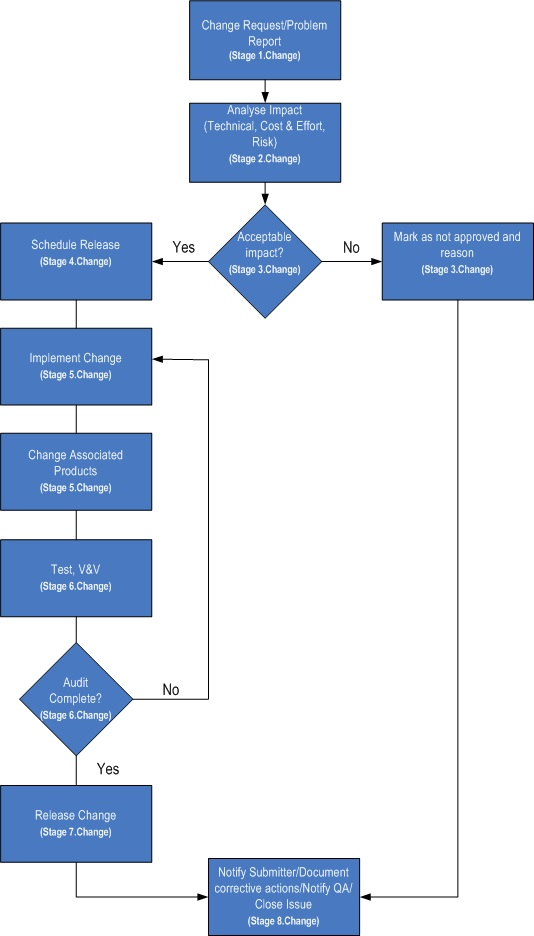
\includegraphics{./figures/ChangeProblemManagementProcess.JPG}
\caption{Change/Problem Management Process flow}
\end{figure}


\subsubsection{Stage One: Change Request/Problem Report}

\begin{itemize}
\item The Change Requester/Problem Reporter has the responsibility of
documenting and submitting the Change Request/Problem Report.
\item Problem and Change requests notified to Change/Problem Owner 
\item The Change Request shall contain the following items:
\begin{itemize}
\item definition of the scope: 
\begin{itemize}
\item \underline{\it stand alone}: The bug or change request mainly affects one phase of the life-cycle (e.g erroneous development of the activities of a phase)
\item \underline{\it cross-institutional}: The bug or the change request has an impact on different phases of the development life-cycle (e.g missing or erroneous specification).
\end{itemize}
\item identification of the products impacted:
\begin{itemize}
\item software
\item formal specification
\item model
\item documentation
\item others
\end{itemize}
\item priority: 
\begin{itemize}
\item \underline{\it immediate}: The bug or the change request should be resolved immediately
\item \underline{\it high}: This bug or the change request should be resolved as soon as possible in the normal course of development activity, before the software is released. 
\item \underline{\it medium}: This bug or the change request should be repaired after serious bugs or emergency change requests have been fixed. 
\item \underline{\it low}: It can be resolved in a future major system revision or not be resolved at all.
\end{itemize}
\item classification: 
\begin{itemize}
\item bug
\item enhancement
\item new requirements
\item change
\end{itemize}
\item severity: 
\begin{itemize}
\item \underline{\it critical}: The bug causes a failure of the complete software system, subsystem or a program within the system
\item \underline{\it high}: The bug does not cause a failure, but causes the system to produce incorrect, incomplete, inconsistent results or impairs the system usability. 
\item \underline{\it medium}: The bug does not cause a failure, does not impair usability, and does not interfere in the fluent work of the system and programs. 
\item \underline{\it low}: The bug is an aesthetic, is an enhancement or is a result of non-conformance to a standard.
\end{itemize}
\item Any additional information that is vital to understand the change/problem must be included when defining it.
\end{itemize}
\item The Problem/Change Request will be assigned a unique Id. Code, and will be assigned the status of “Open”
\item The Change/Problem Owner will perform a first review (completeness, accuracy, scope, severity, priority, classification) of the information provided.
\item All comments will be made and answered using the Change/Problem Management Tool 
\item The Change/Problem Owner will be redirect the request to the relevant parties within the Change/Problem Review Team for further analysis. If needed, additional information will be requested.
\end{itemize}

\subsubsection{Stage Two: Perform Impact Analysis}

\begin{itemize}
\item The receiving parties will assess the impact of the Problem/Change Request. Depending on the scope of the request, the Change/Problem Owner will engage all or only some of the members of the Change/Problem Review Team. 
\item Each Product Owner must have predetermined individuals responsible for reviewing all Change Requests/Problems Report that have specified their group as member of Change/Problem Review Team. This resource is responsible for reviewing all changes affecting their group. The resource will assess the impact on their group and notify all members of the Change/Problem Review Team.
\item The integration of the Configuration Management Tool and the Change/Problem Management Tool will help the Team in performing a proper impact assessment
\item The individual impact assessments (IA) will be registered in the Change/Problem Management Tool, compiled and analysed by the Change Owner
\item A Change Request should be evaluated in terms of required corrective action or system enhancement, technical design, risk and impact analysis, and business case.
\item The impact analysis of the change/problem report should cover the following:
\begin{itemize}
\item \underline{\it technical impact}: The Change/Problem Review Team  should estimate the effort of implementing the changes or problem resolution. 
\item \underline{\it economic impact}: The Change/Problem Review Team  estimates the effort needed and the cost of both implementation and not implementation of the change/problem
\item \underline{\it scope impact}: 
\item \underline{\it planning impact}: The Change/Problem Owner with support of Change/problem reviewers should estimate how the implementation of the change or problem resolution affects to the schedule and propose the best option or release to implement it.
\end{itemize} 
\end{itemize}

\subsubsection{Stage Three: Accepts/Rejects Change}

\begin{itemize}
\item In case of change requests with a clear cross-institutional impact, the impact assessment (IA) will be submitted to the CCB for approval.
\item The CCB will be responsible for approving or rejecting these types of changes and assisting in the assessment and prioritization of changes
\item The CCB should balance the need for change with the need to minimize inherent risks.
\item In the case of bugs or minor change requests, the impact assessment IA will be assessed by the Change/Problem owner
\item In case the Problem/Change request is not accepted, the Change Owner will include the reason in the Change/Problem Management Tool and the issue will be closed. 
\item The CCB members should selectively be chosen to ensure that the requested changes are thoroughly checked and assessed from both a technical and business perspective
\item The Change Requester will be informed about the decision taken
\end{itemize}

\subsubsection{Stage Four: Schedule Release}
\begin{itemize}
\item The Change/Problem Owner schedules the development of the authorized change based on impact analysis results.
\item The Change/Problem Owner will allocate the appropriate resources to the implementation of the change/problem incorporating the new necessities detected during the impact assessment of the specific change/problem (resources, effort/time, equipment, tools, training, tasks/products dependences and/or task additions/deletions) into the existing schedule to produce a new project schedule.
\end{itemize}

\subsubsection{Stage Five: Change Implementation}
\begin{itemize}
\item In case of major changes, prior to the implementation, the implementer should prepare a backout plan to include:
\begin{itemize}
\item A detailed step-by-step procedure for reversing the change
\item Time needed to perform the back out
\item Back out risk
\item A plan to mitigate the severity of any potential negative impact resulting from implementation reversal
\item Detailed testing plans
\end{itemize}
\item The Implementer should follow the implementation action items detailed in the Change Request/Problem Report. Any deviation from the approved implementation plan must be approved by the CCB or Change/Problem Owner depending of the type of the change (See {\it{Stage Three: Accepts/Rejects Change})}
\item As the implementation is performed,
\begin{itemize}
\item the identification code of the problem/change request will be referenced in the configuration items as they are modified, 
\item the Change/Problem Management Tool will register the details (CI, scope) of the problem resolutions activities performed
\end{itemize}
\item As soon as the implementation plan is finalised, the status of the Problem/Change Request will be “Fixed” and therefore ready for auditing
\end{itemize}

\subsubsection{Stage Six: Test Change/problem}
\begin{itemize}
\item The implementation will be audited by the tester and the issue will become either resolved or re-open
\item The tester must determine the success of the change/problem based on execution of the post implementation test plan and success criteria identified in the Change Request/Problem Report. If the change was not
completed successfully as planned or is incomplete, the tester should re-open the issue and all parties impacted by the unsuccessful completion of the change must be notified.
\item The information regarding the success/failure of tests
should be included in the Change Request/Problem Report.
\item The Change Review Team will perform periodical audits and quality assessments of the bugs and change requests received. 
\begin{itemize}
\item Audits to verify the process itself.
\item Quality Assessments to verify the evolution of the product quality. 
\end{itemize}
\end{itemize}

\subsubsection{Stage Seven: Release Change}
\begin{itemize}
\item The Change Owner will publish/launch the new release
\end{itemize}

\subsubsection{Stage Eight: Close Issue}
\begin{itemize}
\item The Change/Problem Owner closes the Change Request/Problem Report
\item The Change Requester, Change Review Team and CCB will be notified
\end{itemize}

\section{ANNEXES - Technical Instructions for using the Change/Problem Management tool}


\end{document}
